%0.5 Seiten
\chapter{Sensorik, Aktorik und andere Hardware}
Was eine Autonome Paketdrohne anspruchsvoller als eine herkömmliche Drohne mit Fernbedienung macht, ist vor allem die Fähigkeit, selbstständig sich zurechtzufinden und ihre Aufgabe ohne die Hilfe von Menschen zu erledigen. Um mit der Umgebung zu interagieren braucht man Sensoren, welche zur Wahrnehmung sprich zur Messung und Kontrolle von Umgebungsvariablen dienen, als auch Aktoren, welche letztendlich die Umgebung, gesteuert durch elektrische Signale, beeinflussen können. Die Sensoren sind also die Sinne, wie zum Beispiel: fühlen, sehen oder auch riechen, welche der Drohne zur Verfügung stehen, wobei die Aktorik die Arme und Beine der Drohne sind. Um also eine Drohne zu entwickeln, welche sich filigran wie eine Katze bewegt und nicht etwa wie ein Elefant braucht man dementsprechend präzise Sensorik und Akorik.


%1 Seite
\section{Sensorik}

%1 Seite
\subsection{Positionssensorik}
Die Position eines Objektes kann man entweder relativ, also in relation zu einem anderen Objekt angeben oder man gibt die Position absolut an, wie zum Beispiel bei einem GPS in Längen- und Breitengrad. Wir haben uns dazu entschieden einen Mischung aus beidem zu benutzen, da man so eine besonders hohe Genauigkeit erreichen kann.
\\
\\ Da die Drohne Pakete ausliefern können soll, brauchen wir dementsprechend einen Sensor welcher eine absolute Position wiedergibt. Um die absolute Globale Position zu bestimmen gibt es nur eine sinnvolle Möglichkeit und zwar GPS, was für Global Positioning System steht und weltweit funktioniert. Da GPS Sensoren allerdings nur auf etwa 10 Meter genau sind und wir Pakete mit einer genauigkeit von etwa +-5cm anfliegen wollen ist die Positionsbestimmung über GPS nicht ausreichend. Somit müssen wir weitere Sensoren zur Unterstützung verwenden. Zur genauen Lokalisiernung des Pakets verwenden wir eine Kamera, die, wie in dem Kapitel Bilderkennung beschrieben, durch Bilderkennung die genaue Position des Pakets ermittelt. Durch die Kamera lässt sich die Drohne sehr gut mittig über dem Paket Platzieren, jedoch kann man nicht wirklich gut die höhe aus einer einzelnen Kamera bestimmen. Um die Höhe genau zu bestimmen bräuchte man entweder eine Stereokamera oder einen Abstandssensor, für welchen wir uns aus Kostengründen entschieden haben.

%1 Seite
\subsection{Ultraschallsensor}
Zur bestimmung von Abständen gibt es mehrere Ansätze, mit unterschiedlichen Vor- und Nachteilen. Man kann den Abstand über die Signallaufzeit, Triangulation oder auch über die Phasendifferenz bestimmen. Am Häufigsten sind dabei die Signallaufzeitsensoren, welche ein Sendeimpuls abgeben und die Zeit bis zu dem Echo messen. Diese Art der Sensoren lässt sich nochmal in drei Unterkategorien einordnen. Es gibt elektromagnetische (wie zum Beispiel Radar), optische (hierzu zählt unter anderem Infrarot und Lidar) und akustische (Beispielsweise Ultraschall) Abstandssensoren, die alle ihre Vor- und Nachteile haben. Wir haben uns für einen Ultraschallsensor entschieden, da dieser in dem von uns gewünschtem Bereich (ca. 2 Meter) auf etwa 10cm genau ist und vorallem weil es ein besonders kostengünstiger Sensor ist. Ein Lidarsensor wäre auch eine gute Alternative, jedoch sind diese Sensoren noch deutlich teurer als herkömmliche Ultraschallsensoren.
\\
\\
Unser Aufbau ist wie in der Abbildung dargestellt, der Eingang des Sensors ist mit einem GPIO OUT Pin verbunden und der Ausgang über einen Spannungsteiler mit einem GPIO OUT verbunden um hier eine Spannung von 3,3V zu erreichen. Außerdem wird noch jeweils Masse mit Masse vom Raspi verbunden und 5V mit den 5V des Raspi verbunden.
\\
In der traditionellen Softwareentwicklung gibt es dafür sogenannte Threads. Diese sind separate Ausführungsstränge, die quasi gleichzeitig ausgeführt werden und sich dann beispielsweise ein Datenobjekt im Speicher teilen und über dieses miteinander kommunizieren können. Das entspricht dann einer Dreischicht-Architektur.
\begin{figure}[h]
	\centering
	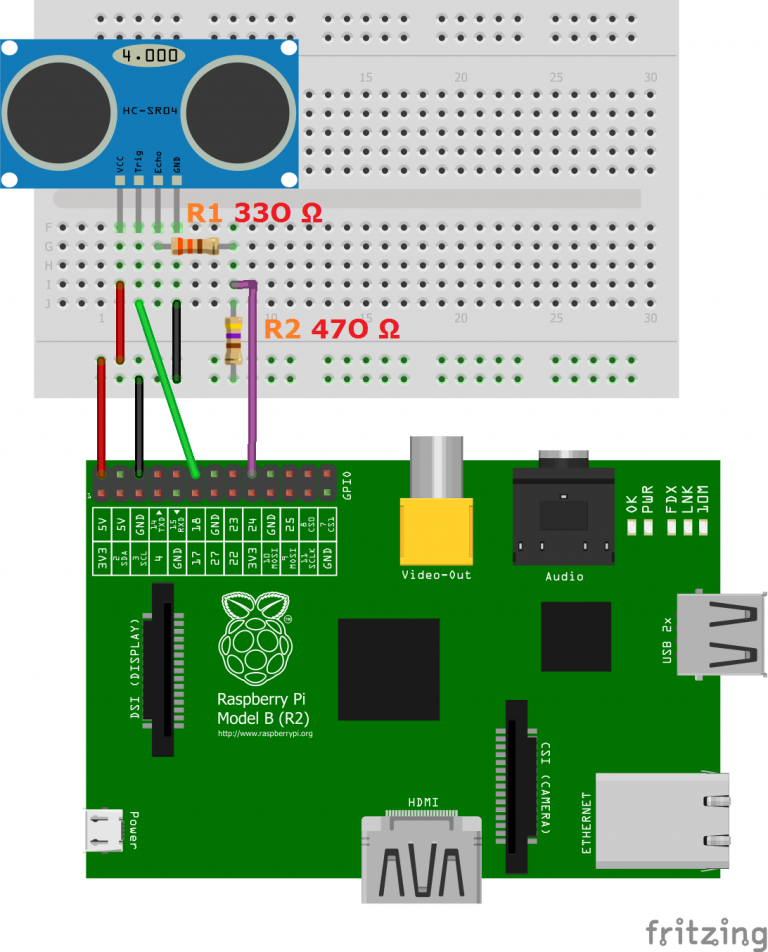
\includegraphics[scale=0.3]{"Grafiken/Ultraschallsensor.png"}
	\caption{Ultraschallsensor Schaubild}
	\label{fig:meine-grafik}
\end{figure}
\\



%1.5 Seiten
\subsection{Global Positioning System (GPS)}
\subsubsection{Funktionsweise}
Wie der Name schon impliziert handelt es sich bei GPS um ein System welches einem die globale Position angibt. Es gibt mehrere solcher Systeme, das jedoch weitverbreitetste ist das NAVSTAR GPS, welches von den Vereinigten Staaten in den 1970er-Jahren entwickelt und bis heute ständig renoviert und in stand gehalten wird. Dieses System besteht momentan aus 31 aktiven Satelliten im Orbit, es werden jedoch nur 24 Satelliten benötigt damit die aktuelle Konstelation funktioniert. Die Überschüssigen Satelliten werden lediglich zur verbesserung der Signalstärke und steigerung der Fehlertoleranz verwendet. Das System ist so asugelegt, dass maan an jedem Üunkt auf der Erde immer Kontakt zu mindestens vier Satelliten gleichzeitig hat. Jeder Satellit sendet in einem Takt von Einer Millisekunde ein Siganl, welches die Position als auch die genaue Uhrzeit des Senders, also des Satellitens, beinhaltet. Mit diesen Daten kann der Empfänger dann seine aktuelle Position, sprich Längen- und Breitengrad als auch seine Höhe berechnen. Normaelrweise sind, um einen Punkt auf der Erde zu bestimmen, nur drei Satelliten notwendig, da aber der Empfänger meist keine ausreichend präzise Uhr besitzt, welche zur berechnung des Standorts benötigt wird, da das Signal mit Lichtgeschwindigkeit unterwegs ist und somit etwa 300 Meter pro Mikrosekunde zurücklegt, wird ein vierter Satellit zum Uhrenfehler ausgleich benötigt. Aus den vier Signalen wird dann über die Signallaufzeit die aktuelle Position berechnet.
\\
\\
Jedoch hat dieses System auch seine Limittierungen, denn sobald der Empfänger keine uneingeschränkte Sicht mehr zu vier Satelliten auf einmal hat, kann er die genaue Position nicht mehr bestimmen. Das Signal von den Satelliten wird relativ schnell von Hochhäusern Brücken oder Tunneln aufgehalten, weswegen wir auch unsere Tests nicht in unserem Labor ausführen konnten, da dort keine stabile GPS Verbidung garantirt ist.

\subsubsection{Hardwareimplementierung}

%1.5 Seite
\subsection{Kamera}

%0.5 Seite
\section{Aktorik}

%1 Seite
\subsection{Hubzylinder}

%1.5 Seiten
\subsection{PX 4}
